% #######################################
% ########### FILL THESE IN #############
% #######################################
\def\mytitle{Coursework 2 - Quiz Application}
%\def\mykeywords{Fill, These, In, %So, google, can, find, your, %report}
\def\myauthor{David Frame}
\def\contact{40200819@live.napier.ac.uk}
\def\mymodule{Advanced Web Technologies (SET09103)}
% #######################################
% #### YOU DON'T NEED TO TOUCH BELOW ####
% #######################################
\documentclass[10pt, a4paper]{article}
\usepackage[a4paper,outer=1.5cm,inner=1.5cm,top=1.75cm,bottom=1.5cm]{geometry}
\twocolumn
\usepackage{graphicx}
\graphicspath{{./images/}}
%colour our links, remove weird boxes
\usepackage[colorlinks,linkcolor={black},citecolor={blue!80!black},urlcolor={blue!80!black}]{hyperref}
%Stop indentation on new paragraphs
\usepackage[parfill]{parskip}
%% Arial-like font
\IfFileExists{uarial.sty}
{
    \usepackage[english]{babel}
    \usepackage[T1]{fontenc}
    \usepackage{uarial}
    \renewcommand{\familydefault}{\sfdefault}
}{
    \GenericError{}{Couldn't find Arial font}{ you may need to install 'nonfree' fonts on your system}{}
    \usepackage{lmodern}
    \renewcommand*\familydefault{\sfdefault}
}
%Napier logo top right
\usepackage{watermark}
%Lorem Ipusm dolor please don't leave any in you final report ;)
\usepackage{lipsum}
\usepackage{xcolor}
\usepackage{listings}
%give us the Capital H that we all know and love
\usepackage{float}
%tone down the line spacing after section titles
\usepackage{titlesec}
%Cool maths printing
\usepackage{amsmath}
%PseudoCode
\usepackage{algorithm2e}

\titlespacing{\subsection}{0pt}{\parskip}{-3pt}
\titlespacing{\subsubsection}{0pt}{\parskip}{-\parskip}
\titlespacing{\paragraph}{0pt}{\parskip}{\parskip}
\newcommand{\figuremacro}[5]{
    \begin{figure}[#1]
        \centering
        \includegraphics[width=#5\columnwidth]{#2}
        \caption[#3]{\textbf{#3}#4}
        \label{fig:#2}
    \end{figure}
}

\lstset{
	escapeinside={/*@}{@*/}, language=C++,
	basicstyle=\fontsize{8.5}{12}\selectfont,
	numbers=left,numbersep=2pt,xleftmargin=2pt,frame=tb,
    columns=fullflexible,showstringspaces=false,tabsize=4,
    keepspaces=true,showtabs=false,showspaces=false,
    backgroundcolor=\color{white}, morekeywords={inline,public,
    class,private,protected,struct},captionpos=t,lineskip=-0.4em,
	aboveskip=10pt, extendedchars=true, breaklines=true,
	prebreak = \raisebox{0ex}[0ex][0ex]{\ensuremath{\hookleftarrow}},
	keywordstyle=\color[rgb]{0,0,1},
	commentstyle=\color[rgb]{0.133,0.545,0.133},
	stringstyle=\color[rgb]{0.627,0.126,0.941}
}

\thiswatermark{\centering \put(336.5,-38.0){
\includegraphics[scale=0.8]{logo}} }
\title{\mytitle}
\author{\myauthor\hspace{1em}\\\contact\\Edinburgh Napier University\hspace{0.5em}-\hspace{0.5em}\mymodule}
\date{}
\hypersetup{pdfauthor=\myauthor,pdftitle=\mytitle,pdfkeywords=\mykeywords}
\sloppy
% #######################################
% ########### START FROM HERE ###########
% #######################################
\begin{document}
    \maketitle
    %\begin{abstract}
    %    %Replace the lipsum command with actual text 
    %    \lipsum[2]
    %\end{abstract}
    
    %\textbf{Keywords -- %}{\mykeywords}
    
    \section{Introduction}

    This report will discuss and evaluate the quiz application, explore options for expansion and look at the author's process for creating the application.
    
    The quiz application allows admin users to create rooms, add and edit questions (see figure \ref{questionEditScreen}) and then host quiz games for many other users. 
    
    When users log into a room (see figure \ref{enterScreen}) using the room code and a username, their name will be added to the lobby (see figure \ref{lobbyScreen}) on the admin user's screen, which would be on a television or projected for the other users to see. 
    
    The users are sent to a wait screen that polls once per second until the admin starts the quiz - at which point they will enter the quiz page on the first question (see figure \ref{quizScreen}).
    
    After answering a question, the wait screen appears again until everyone has answered, it then moves on to the next question. This process continues until the last question where it will redirect to the results screen, where the players are ordered based on their score (see figure \ref{resultsScreen}).
    
    %\figuremacro{h}{HomeScreen.PNG}{Home Screen}{ - An unfiltered list of games}{1.0}
    %You should cite References like this: \cite{Keshav}. The references are saved in an external .bib file, and will automatically be added to the bibliography at the end once cited.
    
	\section{Design}
	The URL hierarchy for this application is mostly horizontal due to the back and forth nature of the application's use case.
	
	As an example, the admin currently must go via the question edit screen to enter a lobby, but an option to go straight to the lobby from the admin screen would make sense as a future addition - so having the questionedit page in the hierarchy before the lobby wouldn't always make sense.
	
	See the diagram (figure \ref{URLHierarchy}) for a view of the URL hierarchy. The root (/) redirects to the entry screen for users who are participating in the quiz, while /admin is the entry point for admin users. There are various routes used to run methods on the back end, though these are not shown on the hierarchy.
	
	User accounts were not used for this application, so data security and privacy are mostly non-issues; this could potentially be abused though, as explained in the enhancements section.
	
	\section{Enhancements}
	This application achieves the main goal of creating quiz games that can be played by large groups at a time. However, there is a lot of room for expansion, which will be explored in this section.
	
	\subsection{Protect rooms with a password}
	One of the goals of this project was to make the process of creating, editing and entering rooms as painless as possible. For this reason, user accounts were not used.
	
	This has various benefits, for example removing the concern about the data protection act as no private data is collected.
	
	The only issue with this approach is that anyone with the room code, such as everyone playing in the room, can view and edit the questions.
	
	The easiest way to add security would be an optional password field on the question edit screen, and a password field on the admin screen. 
	
	Doing this wouldn't impact the flow of creating rooms as if an unrecognized room code is entered, a new room would be generated with a blank password. The admin could then add one which would be required the next time, or leave it blank.
	
	\subsection{More options for questions}
	Similar quiz applications like Kahoot have an option for multiple correct answers per question, along with other features like header images for each question.
	
	The questions could be expanded in other ways too, for example integrating multimedia like video and audio into the questions, or even each answer.
	
	On the other hand, the text only approach is very simple, so it would be important to ensure new features don't spoil this advantage.
	
	\subsection{Integrate a Database}
	Currently, the data is stored using Python pickle. The application would need some form of database for a public release as every room is currently loaded by the server for each user - which is not scale-able. 
	
	\subsection{Better results}
	As this application is designed to be used by a group of people, it was tested by the author with some friends. 
	
	The feedback was generally positive, the application ran smoothly with no errors. Some improvements were suggested, mainly relating to player feedback.
	
	The users wanted to see the correct answer after answering a question, they also wanted a better results screen with scores shown along with a summary of the questions.
	
	\subsection{Time limited questions}
	Questions currently have no time limit, which could be seen as a positive or negative depending on the use case. An optional timer with adjustable length would make the application better in situations where an admin expects users to misbehave or disconnect frequently - as the questions could keep going even if some users don't answer. 
	
	A 'next question' button on the admin user's screen would be another solution to this issue.
	
	\section{Critical Evaluation}
	
	This application was quite ambitious - it hinges around real time communication between a host computer and an unlimited number of participants on mobile devices.
	
	The application works very well, with fast response times for users on mobile devices and instant loading for the host.
	
	The target audience was split into admin users and regular users, so the screens were designed to fit the group who would be interacting with them. For example, the quiz screen is quite playful with bright colours and gradients to engage with players, whilst the admin screens are toned down and designed to be used for longer periods - specifically incorporating a dark colour scheme for reduced eye strain.
	
	Creating rooms is as simple as entering a room code, which acts as a password until the lobby is opened and the room code is shown to the participants. Allowing the admin to choose a room code, as opposed to random generation used by similar applications, also gives a degree of personalisation and theming to the quiz.
	
	The question editor is very easy to use and allows for adding and deleting questions, adding and deleting answers on existing questions and changing the correct answer.
	
	Unfortunately, the question screen refreshes after every edit, which could be irritating if a lot of edits needed to be made to a question beyond the bottom of the viewport. This could be improved by editing the questions in JavaScript and using Jinja to show the changes in real time without a page refresh.
	
	The application's logic is almost entirely in the back end, making the application fast and responsive for users on a wide variety of devices. The UI is also flexible and scalable to allow users to join on anything from a PC to a phone.
	
	Python pickle was used due to difficulty implementing the data structure in JSON, the format the author originally intended to use. This ended up being a good decision as it allowed for quick and easy changes to the data structure without needing to update the saving and loading mechanisms. 
	
	The downside to this approach is the reliance on a specific format that only works in Python - which could limit options if JavaScript needed to be used in the future. The author believes this to be a non-issue as the code could simply be replaced with a JSON alternative if necessary, and in the meantime the code is much simpler.
	
	The results and admin screens are very simple as the target audience could be very wide, including people who may not have much experience with back end systems. But with careful consideration of the target audience, these screens could have more features such as the password protection mentioned in the enhancements section. 
	
	Polling was used to emulate real time communication. It works well and is fast for all participants, but a web sockets implementation would make response times even better. It would also reduce data usage, which could be a concern if users were using a cellular network to participate.
	
	\section{Personal Evaluation}
	This application was very challenging to create due to the many systems that needed to work together.
	
	One of the most important aspects of the quiz application is the use of real time communication. The author had no prior experience with this type of web development, so it was a difficult learning curve and took a lot of time to get right. Thankfully, the application was very fun to develop, which helped motivate the author through this process.
	
	Implementing a saving option for the room list took a lot of trial and error due to the complex nesting of custom objects. As previously mentioned, the author intended to use JSON which proved incredibly difficult and a lot of research on the internet didn't help. Eventually the author discovered Python pickle \cite{UsingPickle}, which was a lot simpler and didn't require too much code to implement \cite{PickleImplementation}.
	
	Other than the aforementioned issues, the development process went according to plan, in some cases even exceeding what the author originally planned - such as the ability to create new rooms immediately with no more setup than editing an existing one. The application was fun to develop and was a great opportunity to improve the author's skillset with web technologies. It will definitely be developed more in the future and used as a portfolio piece.
	
\bibliographystyle{ieeetr}
\bibliography{references}

\begin{figure*}
\section{Appendices}
\end{figure*}

\begin{figure*}
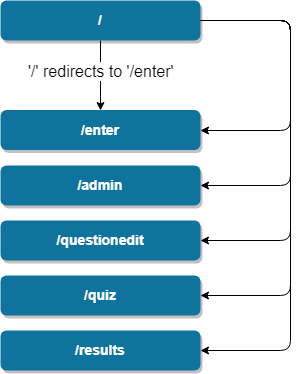
\includegraphics[width=\textwidth]{URLHierarchy.png}.PNG}
\caption[width=\textwidth]{URL Hierarchy - The URL structure of the web app} \label{URLHierarchy}
\end{figure*}

\begin{figure*}
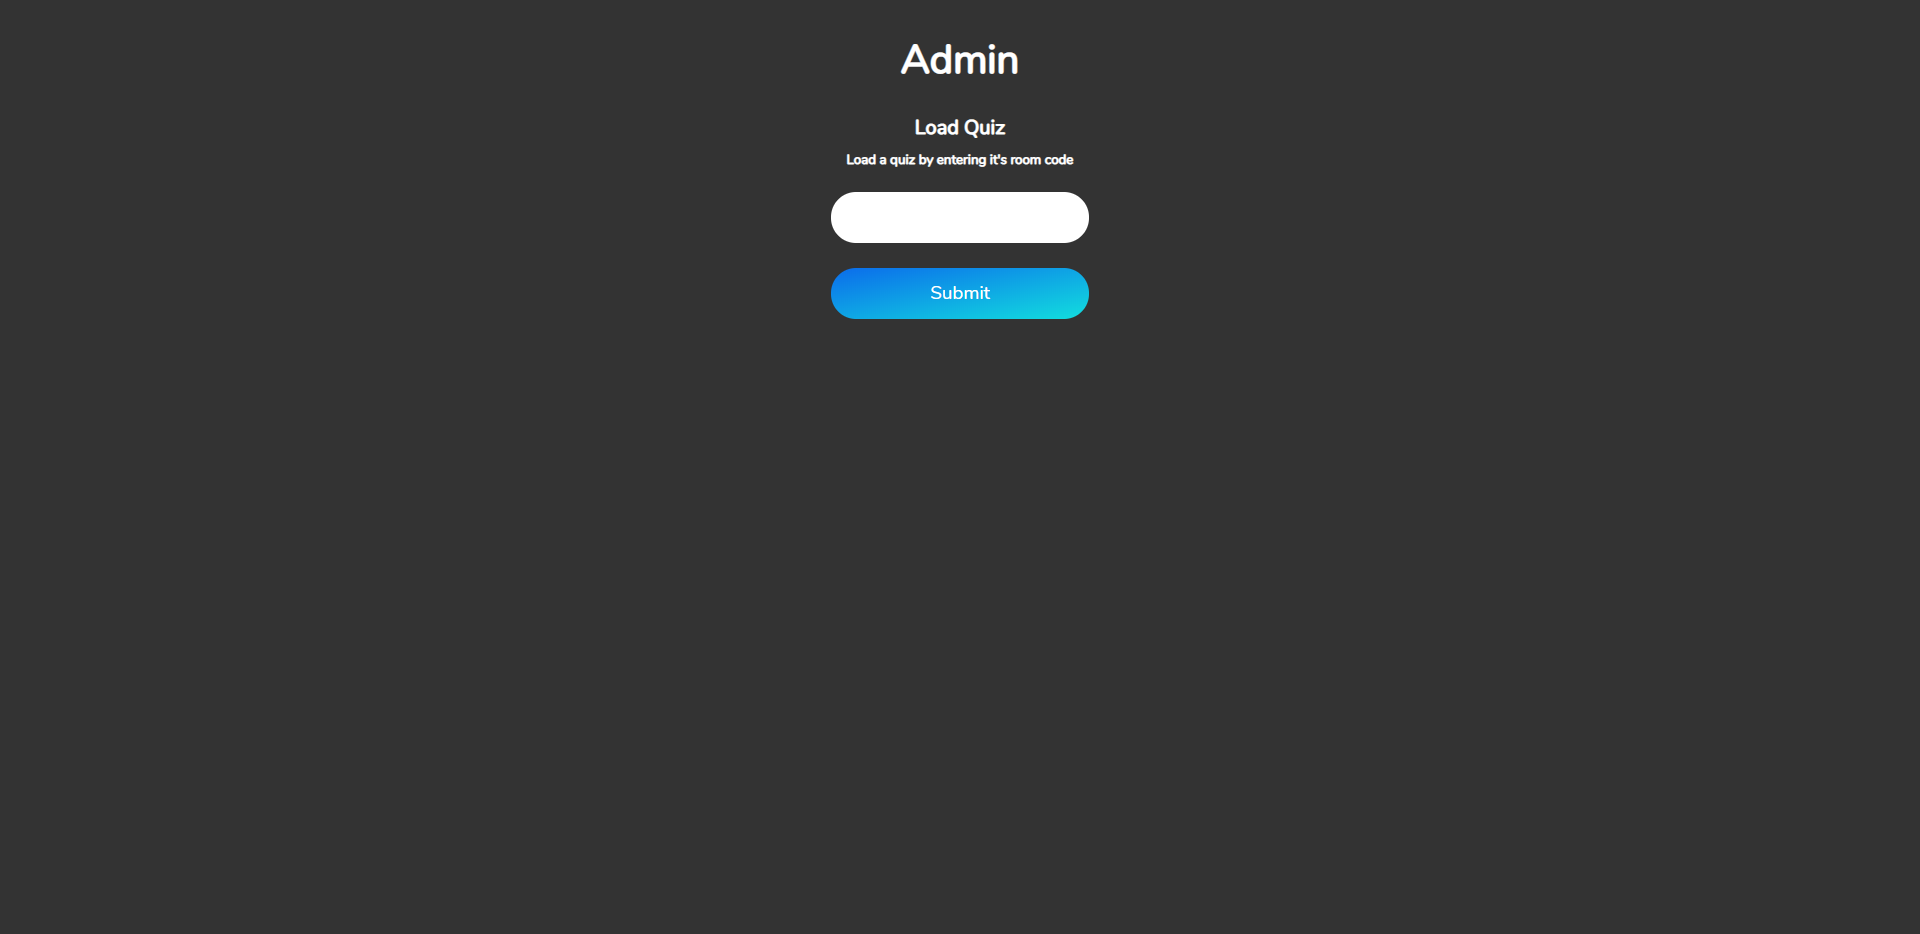
\includegraphics[width=\textwidth]{adminScreen.PNG}
\caption[width=\textwidth]{Home Screen - An unfiltered list of games} \label{adminScreen}
\end{figure*}

\begin{figure*}
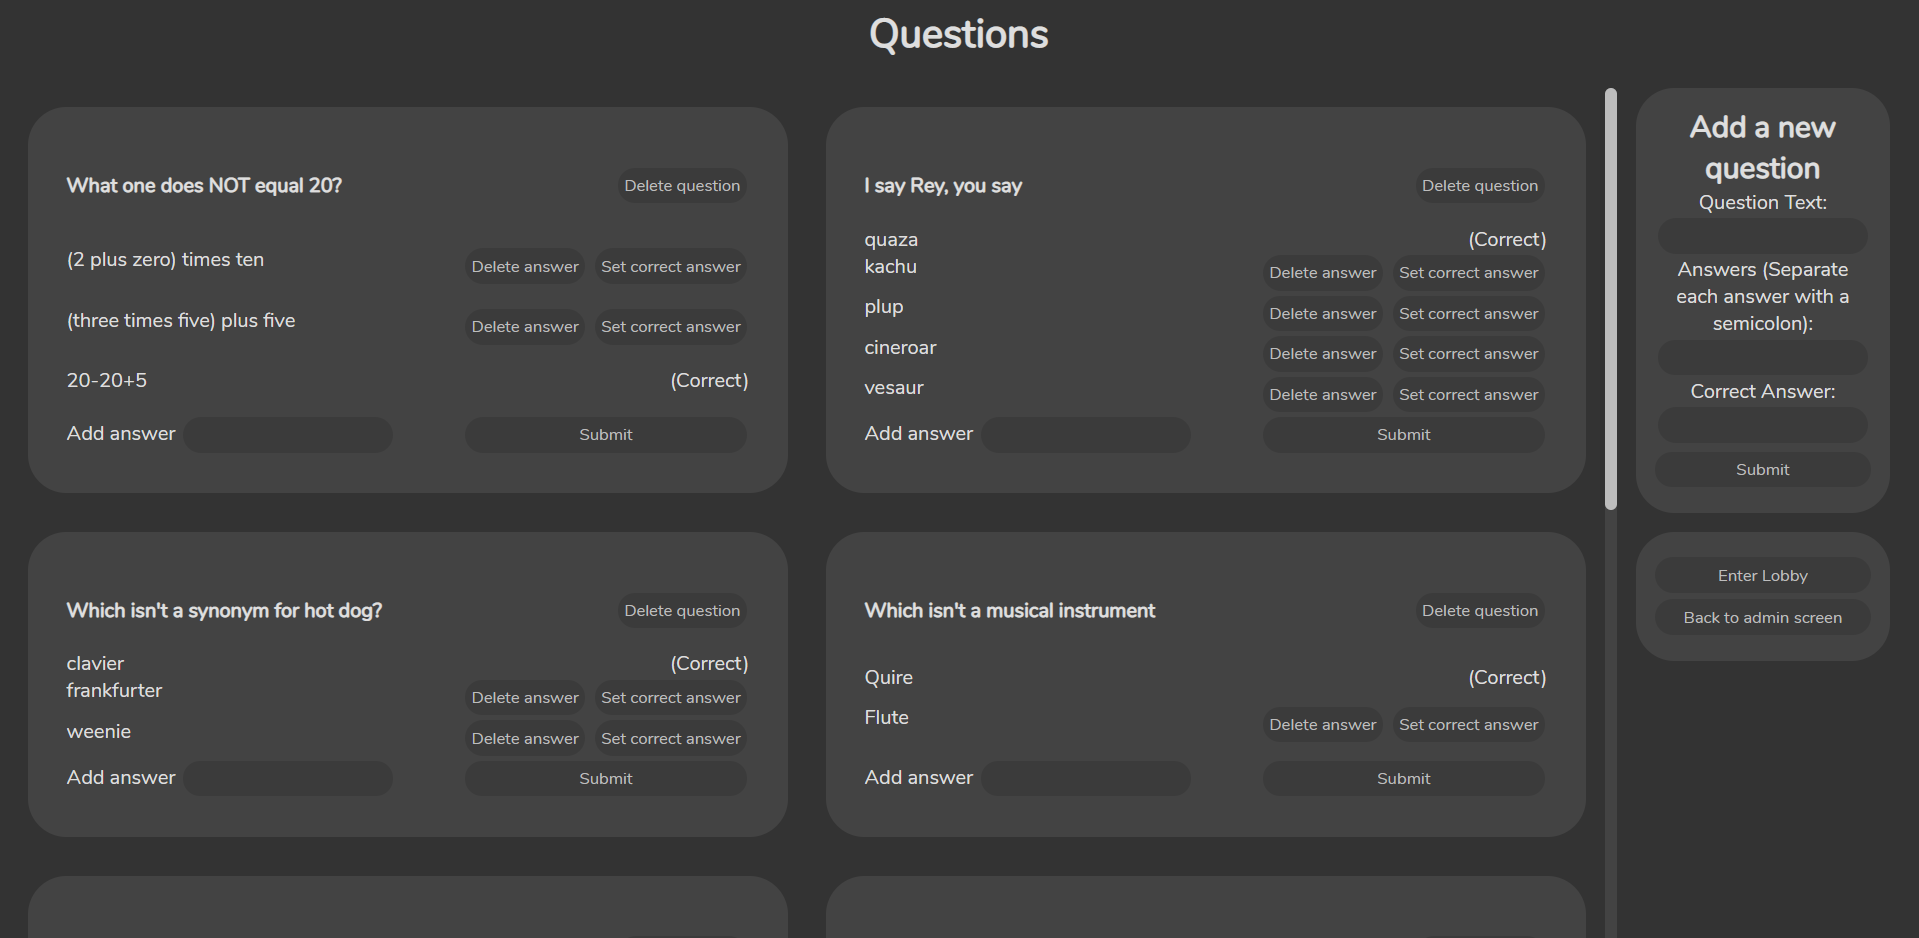
\includegraphics[width=\textwidth]{questionEditScreen.PNG}
\caption[width=\textwidth]{URL Hierarchy - The URL structure of the web app} \label{questionEditScreen}
\end{figure*}

\begin{figure*}

\includegraphics[width=\textwidth]{lobbyScreen.PNG}
\caption[width=\textwidth]{URL Hierarchy - The URL structure of the web app} \label{lobbyScreen}
\end{figure*}

\begin{figure*}
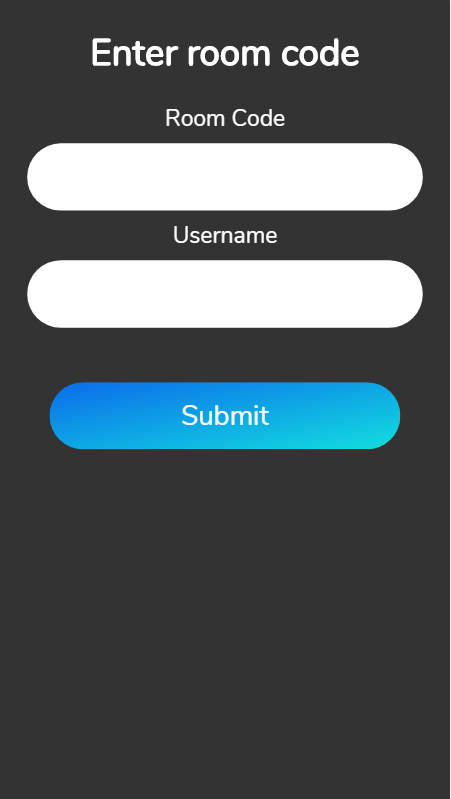
\includegraphics[width=8cm]{enterScreen.PNG}
\caption[width=10cm]{URL Hierarchy - The URL structure of the web app} \label{enterScreen}
\end{figure*}

\begin{figure*}
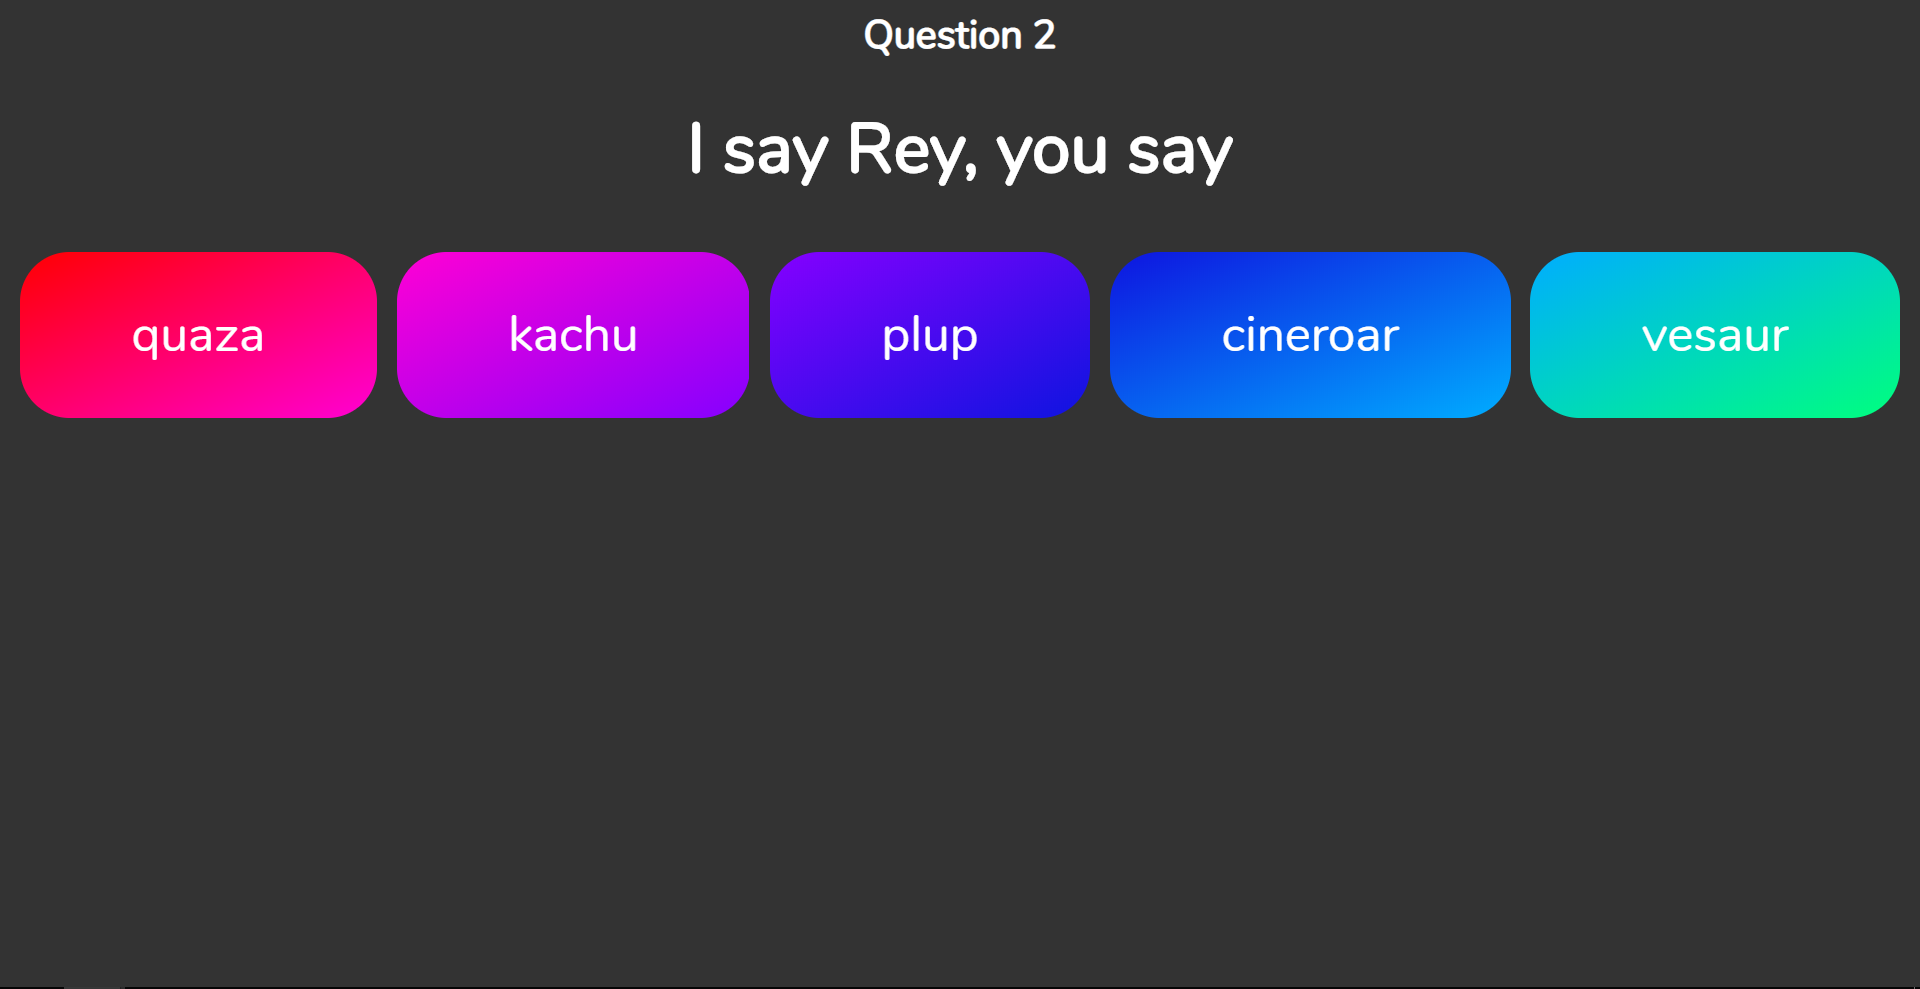
\includegraphics[width=\textwidth]{quizScreen.PNG}
\caption[width=\textwidth]{URL Hierarchy - The URL structure of the web app} \label{quizScreen}
\end{figure*}

\begin{figure*}
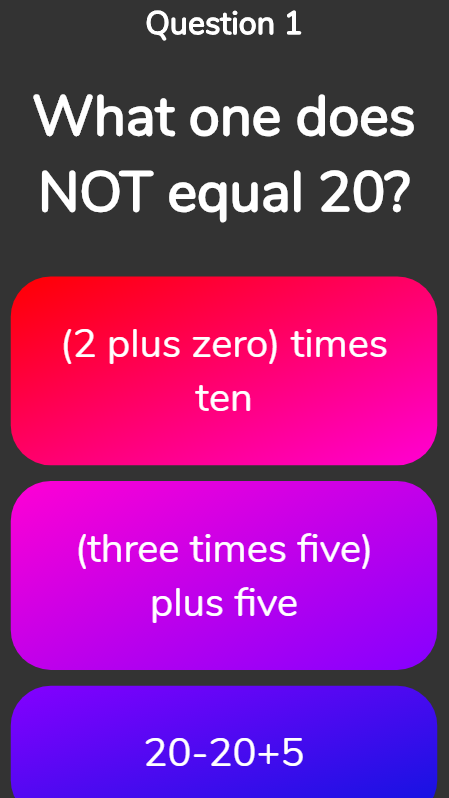
\includegraphics[width=8cm]{quizScreenM.PNG}
\caption[width=10cm]{URL Hierarchy - The URL structure of the web app} \label{quizScreenM}
\end{figure*}

\begin{figure*}

\includegraphics[width=\textwidth]{resultsScreen.PNG}
\caption[width=\textwidth]{URL Hierarchy - The URL structure of the web app} \label{resultsScreen}
\end{figure*}

\end{document}